\documentclass[UTF8,9pt]{ctexart}  %使用中文版的article文档类型排版,并选择UTF8编码格式

% load packages
% Load packages according to your needs

\usepackage{amsmath}
\usepackage{amssymb}
\usepackage[noend]{algpseudocode}
\usepackage{algorithm}
\usepackage{algorithmicx}
\usepackage{array}
\usepackage{graphicx}
% 设置插图目录
\graphicspath{{./figs/}}

\usepackage{xcolor}
\definecolor{wheat}{RGB}{245,222,179}   

\setCJKfamilyfont{\CJKsfdefault}{Times New Roman}
\newcommand\timesnewroman{\CJKfamily{\CJKsfdefault}}
\setCJKfamilyfont{\CJKsfdefault}{SIMFANG.TTF}
\renewcommand\fangsong{\CJKfamily{\CJKsfdefault}}
%\setCJKfamilyfont{\CJKrmdefault}{SimSun}
%\renewcommand\songti{\CJKfamily{\CJKrmdefault}}
\setCJKfamilyfont{\CJKsfdefault}{SimHei}
\renewcommand\heiti{\CJKfamily{\CJKsfdefault}}
\usepackage{biblatex}
\usepackage{hyperref}
\hypersetup{
	colorlinks=true,
	linkcolor=blue,
	filecolor=blue,      
	urlcolor=blue,
	citecolor=cyan,
}
\def\equationautorefname{\textbf{公式}}%
\def\algorithmautorefname{\textbf{算法}}% 
\def\tableautorefname{\textbf{表}}%
\def\figureautorefname{\textbf{图}}%
\usepackage{titlesec}
\titleformat{\section}{\centering\LARGE\heiti}{第\,\thesection\,章}{1em}{}
\titleformat{\subsection}{\centering\large\heiti}{第\,\thesubsection\,节}{1em}{}
\titleformat{\subsubsection}{\centering\small\heiti}{\thesubsubsection}{1em}{}
\usepackage{minted}
\usepackage{listings}
\usepackage{color}
\definecolor{dkgreen}{rgb}{0,0.6,0}
\definecolor{gray}{rgb}{0.5,0.5,0.5}
\definecolor{mauve}{rgb}{0.58,0,0.82}

\lstset{ %
	language=python,                % the language of the code
	basicstyle=\footnotesize,       % the size of the fonts that are used for the code
	numbers=left,                   % where to put the line-numbers
	numberstyle=\tiny\color{gray},  % the style that is used for the line-numbers
	stepnumber=1,                   % the step between two line-numbers. If it's 1, each line 
	% will be numbered
	numbersep=5pt,                  % how far the line-numbers are from the code
	backgroundcolor=\color{white},  % choose the background color. You must add \usepackage{color}
	showspaces=false,               % show spaces adding particular underscores
	showstringspaces=false,         % underline spaces within strings
	showtabs=false,                 % show tabs within strings adding particular underscores
	frame=single,                   % adds a frame around the code
	rulecolor=\color{black},        % if not set, the frame-color may be changed on line-breaks within not-black text (e.g. commens (green here))
	tabsize=2,                      % sets default tabsize to 2 spaces
	captionpos=b,                   % sets the caption-position to bottom
	breaklines=true,                % sets automatic line breaking
	breakatwhitespace=false,        % sets if automatic breaks should only happen at whitespace
	title=\lstname,                 % show the filename of files included with \lstinputlisting;
	% also try caption instead of title
	keywordstyle=\color{blue},      % keyword style
	commentstyle=\color{dkgreen},   % comment style
	stringstyle=\color{mauve},      % string literal style
	escapeinside={\%*}{*)},         % if you want to add LaTeX within your code
	morekeywords={*,...}            % if you want to add more keywords to the set
}


% 中英文题目
\title{\heiti\fontsize{22}{\baselineskip} 中文题目 \\ \relax
\timesnewroman\fontsize{22}{\baselineskip} English Title}
\author{
\fangsong\fontsize{16}{\baselineskip} 2019000000·计算机科学与技术·李 \\ \relax
\fangsong\fontsize{16}{\baselineskip} 2019000000·计算机科学与技术·刘 \\ \relax
\fangsong\fontsize{16}{\baselineskip} 2019000000·软件工程·侯
}  
\date{\today}  

\addbibresource[location=local]{bib/sample.bib}

\begin{document}  %开始写文章     
 	\maketitle

	\newpage
	
	\section{章节名}
	\begin{enumerate}
		\item 参考文献实例。\cite{boss1997uncoupling}
	\end{enumerate}
	
	
	\section{表格效果}

	\begin{table}[htb]
		\centering
		\begin{tabular}{l l l l l}
			\hline
			
			数据集 & 样本数 & 维度 & 类数 & 数据类型 \\ \hline
			MNIST & 3000 & 784 & 10 & 手写体数字 \\ 
			Yale & 165 & 1024 & 15 & 人脸图像 \\ 
			lung & 203 & 3312 & 5 & 生物数据 \\ \hline
			
		\end{tabular}
		\caption{数据集}
	\end{table}



	\section{内容}
	
	\subsection{代码}
		两种输入代码的模板,具体效果如下
		


	\begin{lstlisting}
	clf = GaussianNB()
	clf = clf.fit(dataX_train, dataY_train)
	y_pred=clf.predict(dataX_predict)
	print("高斯朴素贝叶斯,样本总数: %d 错误样本数 : %d" % (dataX_train.shape[0],(dataY_predict != y_pred).sum()))
	print("准确率为: %f" % (1 - (dataY_predict != y_pred).sum()/dataX_predict.shape[0]))
	\end{lstlisting}
	
	
	\begin{minted}[bgcolor=wheat,breaklines=True,firstline=1,firstnumber=1,
	frame=none,linenos=true,showtabs=false,tabsize=4]{c}
		clf = MultinomialNB()
		clf = clf.fit(dataX_train, dataY_train)
		y_pred=clf.predict(dataX_predict)
		print("多项分布朴素贝叶斯,样本总数: %d 错误样本数 : %d" % (dataX_train.shape[0],(dataY_predict != y_pred).sum()))
		print("准确率为: %f" % (1 - (dataY_predict != y_pred).sum()/dataX_predict.shape[0]))
	\end{minted}



		\subsection{公式、算法、表、图}
		公式、算法、表格效果如下,其中使用autoref可以提供公式等的超链接
		
		\autoref{equ:argmax} 公式
		
		\begin{equation}
		\label{equ:argmax}
		\underset{y}{\operatorname{argmax}}\left(\sum_{i: 1 \leq i \leq n \wedge F\left(x_{i}\right) \geq m} \hat{P}\left(y, x_{i}\right) \prod_{j=1}^{n} \hat{P}\left(x_{j} | y, x_{i}\right)\right)
		\end{equation}
		
		\autoref{alg:A} 算法
		
		\begin{algorithm}[htb]
			\caption{算法名称} %算法的名字
			\label{alg:A}
			\hspace*{0.02in} {\bf Input:} %算法的输入, 
			input parameters A, B, C\\
			\hspace*{0.02in} {\bf Output:} %算法的结果输出
			output result
			\begin{algorithmic}[1]
				\State some description % \State 后写一般语句
				\For{condition} % For 语句,需要和EndFor对应
				\State ...
				\If{condition} % If 语句,需要和EndIf对应
				\State ...
				\Else
				\State ...
				\EndIf
				\EndFor
				\While{condition} % While语句,需要和EndWhile对应
				\State ...
				\EndWhile
				\State \Return result
			\end{algorithmic}
		\end{algorithm}
	

		
		如\autoref{tab:machine}所示,为测试表格
		
		\begin{table}[htb]
			\centering
			\caption{测试表格 \label{tab:machine}}
			\begin{tabular}{l l}
				\hline
				硬件 & 配置 \\ \hline
				CPU & Xeon(R) Silver 4116 CPU @ 2.10GHz * 2 \\ 
				显卡 & Tesla P40 \\ 
				内存 & 64GB \\ \hline
			\end{tabular}
		\end{table}
		
	\autoref{fig:singleCNN_2} 测试图片
	
	\begin{figure}[htb]
		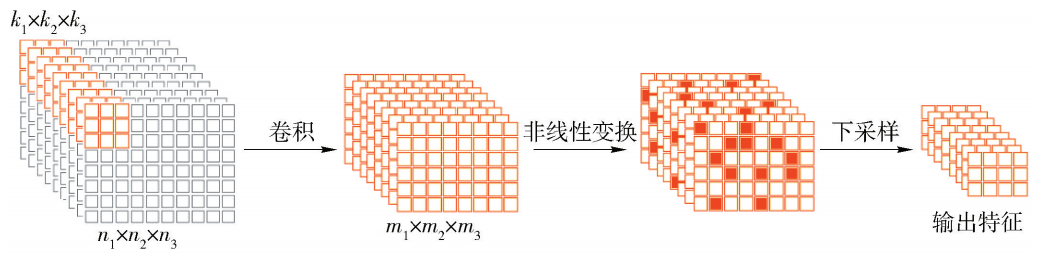
\includegraphics[width=15cm]{example}
		\caption{图片示例}
		\label{fig:singleCNN_2}
	\end{figure}



	\section{学习心得与对话老师}
	\subsection{A}
	这里是心得
	\subsection{B}
	这里是心得
	\subsection{C}
	这里是心得
	

% 排版参考文献表
%\bibliomatter
\printbibliography[heading=bibintoc]%

\end{document}  
